\chapter{Shallow Water 2006 Experiment}
In 2006, from mid-July to mid-September, a large, multi-disciplinary, multi-institution experiment named SW06 was conducted in the New Jersey coast. Part of its goal is to further the understanding of the affects of the nonlinear internal waves on the acoustic propagation in shallow water.

\section{Experiment site and environment moorings}
The SW06 experiment site is approximately 100 miles east of the New Jersey coast (Fig. \ref{fig:mooring}), which is known to generate internal waves during summer time and has been a research testbed for many other experiments before (e.g., SWARM 95). To assess the combined acoustic and oceanographic relationship between the acoustic wave propagation and the internal waves, a total of 62 acoustics and oceanographic moorings were deployed in a 'T' geometry to create an along-shelf path along  the 80 meter isobath and an across-shelf path starting at 600 meters depth and going shoreward to a depth of 60  
meters.  

A cluster of moorings was placed at the intersection of the two paths to create a dense sensor-populated area  
to measure 3-dimensional physical oceanography. Environmental moorings were deployed along both along-shelf and  
across-shelf paths to measure the physical oceanography long those paths. Moorings with acoustic sources were  
placed at the outer ends of the 'T' to propagate various signals along these paths.  Five single hydrophone receivers  
(SHRU) were positioned on the across shelf path and a vertical and horizontal hydrophone array (VLA/HLA) was  
positioned close to the intersection of the 'T' to get large antenna signal receptions from all the acoustics assets that  
were used during SW06.   


There were in total 34 environmental moorings deployed during SW06 experiment to access the physical oceanography of the area. Each of the acoustic moorings (source and receiver) was equipped with thermistors at various depths to help recreate the acoustic channel. Close to the center of the "T" shape mooring layout, a thermistor farm consisting of 16 arrays spacing logarithmically from 0.5 km to 3 km to record the internal waves at different scales. 


Out of 34 environmental moorings, 6 of them were also equipped with Acoustic Doppler Current Profiler(ADCP) to measure the current velocity at the location. The ADCP package including a temperature, conductivity, pressure sensor was locate about 7 meters above the sea floor. The space of measuring bins was set at 1m. The sampling interval of ADCP is 30 seconds and capable of solving internal wave passage but not the fine scale of surface waves. Figure \ref{fig: sw32adcp_temp} shows the current data record by ADCP at mooring SW32 during event 50 in SW06 experiment and the temperature data at the same location. It demonstrates the clear correspondence between the direction and the depth profile of the subsurface current. 
\section{Acoustic moorings}
\subsection{Sources}
During SW06, several acoustic sources were used to transmit sound while environmental data were collected
simultaneously\cite{WHOI}. Here we discuss the acoustic data from a pair of acoustic sources.

\begin{enumerate}
\item Fixed source (NRL300) at mooring SW45

 The source was located 72 m below the sea surface and
10.5 m above the sea floor at $39^{o}10.957'$ N, $72^o56.575'$ W,
and transmitted 2.0489 second Linear Frequency Modulating (LFM)
signals from 270 to 330 Hz every 4 seconds. Transmissions continued
for 7.5 minutes and then repeated every half hour. 
\item Moving source J15 towed by R/V Sharp

There were towed source aboard R/V Sharp of University of Delaware transmitting from 16th Aug. to 20th Aug. Three G34 sources were positioned at depth from 10-30 meters, and one J15 source at approximately 40 meters. The signal transmitted from J15 source (the moving source) will be used in this research. The signal type is Linear Frequency Modulating (LFM) from 100 to 400 Hz every 10 seconds. Transmission continued for 15 minutes in the quiet window of NRL300 source and then repeated every half hour. 


\end{enumerate}
Table \ref{tab:ev50_trans} lists all the transmissions during the internal wave event 50 (explained later) from both the fixed source and the moving source.
\begin{table}
  \centering
  \caption{Transmission during Ev50 from fixed source (NRL300)
    \& moving source (J15)}\label{tab:ev50_trans}
  \begin{tabular}{ccc}
  \hline
  Transmission & Time(GMT) & Source\\
  \hline
  1 & 20:30-20:37 & NRL300\\
  %\hline
  2 &  21:00-21:07 &  NRL300\\
  %\hline
  3 & 21:11-21:26 & J15/R.V. Sharp\\
  %\hline
  4 & 21:30-21:37 & NRL300\\
  %\hline
  5 & 21:41-21:46 & J15/R.V. Sharp\\
  %\hline
  6 & 22:00-22:07 & NRL300\\
  %\hline
  7 & 22:11-22:26 & J15/R.V. Sharp\\
  %\hline
  8 & 22:30-22:37 & NRL300\\
  %\hline
  9 & 22:41-22:56 & J15/R.V. Sharp\\
  %\hline
  10 & 23:00-23:07 & NRL300\\
  %\hline
  11 & 23:11-23:16 & J15/R.V. Sharp\\
  %\hline
  12 & 23:30-23:37 & NRL300\\
  \hline
  \end{tabular}
\end{table}

\subsection{Receiver array}
 A vertical and
horizontal receiver array (the "Shark VHLA") on mooring SW54 was
located at $39^o01.252'$ N, $73^o02.983'$ W, about 20.2 km south of
the NRL source.  The vertical part ('VLA') of the receiver array consisted
of 16 hydrophones with 3.5 m spacing and was positioned in the water
column from 13.5 m to 77.75 m below the surface. The horizontal part ('HLA')
of the array consisted of 32 hydrophones on the seafloor with
spacing of 15 m, providing 478 m of horizontal aperture. The
sampling rate of the array was 9765.625 Hz. The acoustic track and
the locations of the source and receiver as well as the horizontal
and vertical array configurations are shown in Fig. 1. The water
depth along the acoustic track was about 80 m.

Figure \ref{fig:ship_track_radar} shows the fixed source(NRL300), the receiver array(Shark VHLA) and the semi-circular track of R/V Sharp, who was towing the moving source J15 in the internal wave event 50. Zone 1-5 marks the location of J15 in the transmission windows of J15 in event 50.

\section{Internal wave observation}
The SW06 site is known for generating internal waves. Figure \ref{fig:radarsat} shows a radar image of the ocean taken by Canadian satellite RADASAT over the experimental site near the edge of the continental shelf. The picture shows about 8-10 groups of internal wave packages running from south-east to north-west diagonally, with the wave fronts
approximately parallel to the edge of the continental shelf.  The wave packages are generate at the shelf break ( about 200 m in depth), propagate towards the coast and dissipated at about 50 m. The separation between individual wave packages are approximately 10-20 km. Notice the sever curvature caused by the Hudson Canyon and numerous collisions between wave packages.

Although bearing the word "internal" in its name, internal wave can be visible to a electromagnetic radiation recording device such as a camera or a radar. Together with other factors like wind, surface waves, The subsurface current caused by internal waves changes the equilibrium surface and generates an alternating region of rougher or smother than the average surface scattering the electromagnetic wave differently\cite{intro_apel_1995}\cite{intro_Kropfli_1999}. The image captured by radar or optical device mirrors the current under the surface. During SW06, two research vessels, R/V Oceanus from Woods Hole Oceanography Institution (WHOI) and R/V Sharp from University of Delaware were constantly recording the surface expression of internal waves. 



%\begin{figure}[h]
%\centering
%  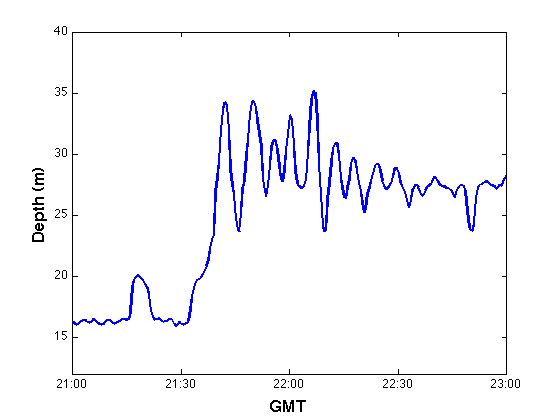
\includegraphics[width=0.8\textwidth]{sw54_aug17_thermocline_18C.png}\\
%  \caption{}
%  \label{fig:sw54_aug17_thermocline_18C}
%\end{figure}
%
%
The passing of internal waves can also be seen by other environmental sensors. 
Figure \ref{fig:sw54_aug17_thermocline_18C_long} shows the depth of $18^o$C thermocline recorded on WHOI VLA (SW54). Before the internal wave, the thermocline is at about 16m, the first soliton wave pushs the thermocline down the 35m, and the later solitons even push further down towards the bottom. There are about 9 distinguishable soliton waves, followed by a long, slow-decreasing tail, the thermocline didn't return to 16m until 6:00 next day - the total duration of internal wave is about 8 hours.


Using an onboard radar of R/V Sharp of University of Delaware, 60 internal wave event were recorded when the surface expressions were visible on the screen during the period of 21 days with various strength and direction. Fig.\ref{fig:IW_dir} shows their angular distribution. The direction spreads from 280-330 degree with respect to north($0^o$), with the strongest peak at about 320 degrees. The propagation paths and the their day rates vary considerably from one wave to another. Lynch {\it et al} \cite{intro_Lynch_2010} reported a similar results by studying satellite imagery. In this study, we focus on a particular internal wave event on August 17, 2006, for which a complete set of acoustic and environmental data were collected simultaneously. In addition, the internal wave surface signatures were
captured continuously by the on-board radars of two research vessels
prior to the arrival of, and during the passing of, the internal wave packet
over the acoustic track.

 

\subsection{Internal wave event 50}
On August 17, 2006, at about 18:00 GMT, the R/V Sharp from the
University of Delaware was located at $38^o59.262'$ N, $72^o57.492'$ W and
the R/V Oceanus from the Woods Hole Oceanographic Institution (WHOI)
was located at $38^o57.426'$ N, $72^o56.676'$ W. Both platforms observed
the origination of the internal wave packet near the shelf break. This event was named
Event 50 on R/V Sharp and Rosey on R/V Oceanus.


Figure \ref{fig:ship_track_radar} show the track of each vessel following this
event from 18:00 GMT on August 17 to 02:00 GMT on August 18, 2006.
The R/V Sharp's track was semi circular, centered at the WHOI
vertical and horizontal line array (Shark VHLA) with the ship being
positioned on the trough of the leading internal wave front and moving with
the advancing front. The R/V Oceanus followed the same internal wave packet
from its initial location, while keeping a watch on the advancing
wave front. Reversals in the track of R/V Oceanus indicate where the
wave packet was crossed, and during these periods, intensive
profiling of temperature, density, turbulence and sound velocity was
conducted.

The two ships observed different parts of the internal wave front, thus
providing a large spatial coverage. The surface signatures of the
internal waves were digitally recorded by on-board ship radar images every 30
seconds. Combined radar images from the two vessels, each about 11.1
km in diameter, covered the receiver and about two thirds of the
acoustic track. 

The direction and speed of the internal wave packet in event 50 can be estimated by measuring the time difference when the leading front arrives at different thermistor arrays, or by averaging the direct measurement from the ship radars. Table \ref{tab-IW_speed} lists the speed and direction estimations by these two methods. A little discrepancy is to be expected.
\begin{table*}[hc]
\caption{ Direction and speed of the internal wave packet in event 50
\label{tab-IW_speed}}
\begin{center} 
\begin{tabular}{ | c|c | c |}
\hline
Data source & IW speed & IW direction\\
\hline
%{\mr{2}{*}{Data source}}& {\mr{2}{*}{Speed} }      & \mc{2}{c|}{Direction}   & {\mr{2}{*}{Signal Type}} & {\mr{2}{*}{Center Freq. }}     \\
%\cline{3-4}
%                 &                 &  Latitude     & Longitude   & &\\\hline \hline
 Thermistor arrays & 0.55m/s & $325^\circ$ \\
 \hline
 Ship radar & 0.60m/s & $330^\circ$\\
 \hline
 
 \hline
 
\end{tabular} 
\end{center}
\end{table*}
%
%

%\subsubsection{Fixed and Moving Sources}
%
%Two WHOI single-frequency sources were deployed in SW06 experiment. The sources were moored in the low water column to excite low mode acoustic propagation. Two Navy Research Lab (NRL) sources were also deployed. These were broadband source transmitting Linear Frequency Modulated signal at 300Hz and 500Hz center frequency. 
%
%\begin{table*}[hc]
%\caption{ Acoustic source moorings in SW06 experiment
%\label{tab-fixed-source}}
%\begin{center} 
%\begin{tabular}{ | c|c | c | c | c |c|}
%\hline \hline
%
%{\mr{2}{*}{Source}}& {\mr{2}{*}{Mooring} }      & \mc{2}{c|}{Location}   & {\mr{2}{*}{Signal Type}} & {\mr{2}{*}{Center Freq. }}     \\
%\cline{3-4}
%                 &                 &  Latitude     & Longitude   & &\\\hline \hline
% WHOI224 & SW47 & $39^\circ 09.2000' N$ & $73^\circ 21.4911'W$& Phase-coded, LFM & 224Hz\\
% \hline
% WHOI400 & SW48 & $39^\circ 09.4534' N$ & $73^\circ 21.3093'W$& Phase-coded, LFM & 400hz\\
% \hline
% NRL300 & SW45 & $39^\circ 10.9574' N$ & $72^\circ 56.575'W$& LFM & 300Hz\\
% \hline
% NRL500 & SW46 & $39^\circ 10.587' N$ & $72^\circ 56.458'W$&LFM & 500Hz\\
% \hline
% 
%\end{tabular} 
%\end{center}
%\end{table*}
%
%The signal transmitted by NRL300 source are the focus of this study. The source linearly swept over 270-330 Hz (chirp) in 2.048 seconds every 4 seconds during the scheduled transmission slot. Each chirp signal contains a 0.2048 seconds amplitude taper at the beginning and the end of the transmission. In addition to NRL300 source, the SW45 mooring was also instrumented with temperature sensors. 
%
%There were towed source aboard R/V Sharp of University of Delaware transmitting from 16th Aug. to 20th Aug. Three G34 sources were positioned at depth from 10-30 meters, and one J15 source at approximately 40 meters. Various types of signal were transmitted: phase-coded, LFG, MIMO etc.   
%
%
%\begin{table*}[hc]
%\caption{ Towed Sources in SW06 experiment
%\label{tab-moving-source}}
%\begin{center} 
%\begin{tabular}{ | c| c | c |c|}
%\hline \hline
%
%Source&Towed by        & Signal Type & Center Freq.      \\
%
%                 \hline \hline
% G34 & R/V Sharp &  Phase-coded, LFM, MIMO & 600Hz\\
% \hline
% J15 & R/V Sharp &  Phase-coded, LFM, MIMO & 200Hz\\
% \hline
% 
%\end{tabular} 
%\end{center}
%\end{table*}
%
%
%%\subsection{Instrumentation}
%%\subsubsection{Source}
%%\subsubsection{Receiver}
%%\subsection{Acoustic Signal}
%%
%%

%
%\begin{table*}[htbp]
%\caption{ IW Events in SW06 experiment 
%\label{tab-sharp}}
%\begin{tabular}{ | c | c | c | c | c | c | c |}
%\hline \hline
%
%{\mr{2}{*}{Event}} &  {\mr{2}{*}{Date}}   & \mc{2}{c|}{GMT}     & \mc{2}{c|}{Location}   & {\mr{2}{*}{Direction }}     \\
%\cline{3-6}
%                   &                      & Start Time & End Time &  Latitude     & Longitude   & \\
%\hline \hline
% 1                 & 02 Aug 2006          & 09:30:00   & 10:48:00  &  $30^\circ 20.6'$ & $-73^\circ 20.6'$   & 325$^{\circ}$\\
%\hline
% 2                 & 02 Aug 2006          & 16:15:00   & 17:24:00 & $39^\circ  4.2'$  & $-73^\circ  1.2'$& 320$^{\circ}$\\
%\hline
% 3                 & 02 Aug 2006          & 22:10:00   & 23:35:00 &     $39^\circ  4.1'$  & $-73^\circ  1.2'$ & 325$^{\circ}$\\
%\hline
% 4                 & 03 Aug 2006          & 06:37:00   & 08:08:00 &     $39^\circ  4.2'$  & $-73^\circ  1.3'$ & 283$^{\circ}$\\   
%\hline
% 5                 & 03 Aug 2006          & 15:26:00   & 16:19:00 &     $39^\circ  5.7'$  & $-72^\circ  58.1'$ & 312$^{\circ}$\\   
%\hline
% 6                 & 03 Aug 2006          & 18:10:00           &19:00:00          &  $39^\circ  5.6'$  & $-72^\circ  58.1'$& 288$^{\circ}$\\   
%\hline
% 7                 & 04 Aug 2006          & 00:45:00   & 01:33:00 &     $39^\circ  5.7'$  & $-72^\circ  58.2'$ & 294$^{\circ}$\\   
%\hline
% 8                 & 04 Aug 2006          & 03:57:00   & 06:22:00 &    $39^\circ  5.6'$  & $-72^\circ  58.0'$& 308$^{\circ}$\\   
%\hline
% 9                 & 04 Aug 2006          & 12:15:00   & 15:39:00 &   $39^\circ  5.7'$  & $-72^\circ  58.2'$ & 301$^{\circ}$\\   
%\hline
% 10                & 04 Aug 2006          & 16:40:00   & 19:24:00 &    $39^\circ  5.6'$  & $-72^\circ  58.0'$ & 313$^{\circ}$\\   
%\hline
% 11                & 05 Aug 2006          & 02:45:00   & 03:25:00 &     $39^\circ  6.7'$  & $-73^\circ  0.9'$ & 302$^{\circ}$\\   
%\hline
% 12                & 05 Aug 2006          & 03:41:00   & 05:20:00 &   $39^\circ  6.7'$  & $-73^\circ  1.1'$& 322$^{\circ}$\\   
%\hline
% 13                & 05 Aug 2006          & 11:30:00   & 13:22:00 &     $39^\circ  6.6'$  & $-73^\circ  0.9'$ & 315$^{\circ}$\\   
%\hline
% 14                & 05 Aug 2006          & 17:30:00   & 18:09:00 &     $39^\circ  6.5'$  & $-73^\circ  0.9'$ & 320$^{\circ}$\\   
%\hline
% 15                & 05 Aug 2006          & 19:00:00   & 21:12:00 &   $39^\circ  6.5'$  & $-73^\circ  0.9'$& 315$^{\circ}$\\   
%\hline
% 16                & 05 Aug 2006          & 22:22:00   & 23:09:00 &     $39^\circ  5.4'$  & $-72^\circ  59.0'$ & 320$^{\circ}$\\   
% \hline
% 17                & 06 Aug 2006          & 16:45:00   & 19:04:00 &     $39^\circ  6.3'$  & $-72^\circ  59.2'$& 305$^{\circ}$\\   
%\hline
% 18                & 06 Aug 2006          & 19:55:00   & 21:02:00 &   $39^\circ  6.3'$  & $-72^\circ  59.2'$ & 322$^{\circ}$\\   
%\hline
% 19                & 06-07 Aug 2006       & 21:48:00   & 01:14:00 &   $39^\circ  6.2'$  & $-72^\circ  59.2'$ & 288$^{\circ}$\\   
%\hline
% 20                & 07 Aug 2006          & 03:28:00   & 07:11:00 &    $39^\circ  6.3'$  & $-72^\circ  59.2'$& 288$^{\circ}$\\   
%\hline
% 21                & 07 Aug 2006          & 07:22:00   & 10:25:00 &     $39^\circ  6.3'$  & $-72^\circ  59.1'$ & 312$^{\circ}$\\   
%\hline
% 22                & 07 Aug 2006          & 10:46:00   & 11:22:00 &     $39^\circ  6.3'$  & $-72^\circ  58.7'$ & 298$^{\circ}$\\   
% \hline
% 23                & 07 Aug 2006          & 18:05:00   & 18:51:00 &     $39^\circ  7.0'$  & $-73^\circ  4.6'$ & 308$^{\circ}$\\   
%\hline
% 24                & 08 Aug 2006          & 00:03:00   & 01:43:00 &     $39^\circ  7.0'$  & $-73^\circ  4.6'$ & 340$^{\circ}$\\   
% \hline
% 25                & 08 Aug 2006          & 03:59:00   & 09:30:00 &    $39^\circ  6.9'$  & $-73^\circ  4.6'$ & 306$^{\circ}$\\   
%\hline
% 26                & 08 Aug 2006          & 18:22:00   & 20:48:00 &      $39^\circ  3.8'$  & $-73^\circ  9.1'$ & 300$^{\circ}$\\   
% \hline
% 27                & 09 Aug 2006          & 03:47:00   & 08:00:00 &     $39^\circ  3.8'$  & $-73^\circ  9.1'$ & 278$^{\circ}$\\   
%\hline
% 28                & 09 Aug 2006          & 16:32:00   & 18:40:00 &      $39^\circ  5.2'$  & $-73^\circ  12.1'$ & 330$^{\circ}$\\   
% \hline
% 29                & 09 Aug 2006          & 20:00:00   & 22:30:00 &    $39^\circ  5.2'$  & $-73^\circ  12.1'$ & 322$^{\circ}$\\   
%\hline
% 30                & 10 Aug 2006          & 03:55:00   & 05:30:00 &     $39^\circ  5.2'$  & $-73^\circ  12.1'$& 322$^{\circ}$\\   
% \hline
% 31                & 10 Aug 2006          & 06:30:00   & 09:30:00 &     $39^\circ  5.3'$  & $-73^\circ  12.1'$ & 325$^{\circ}$\\   
%\hline
% 32                & 10 Aug 2006          & 10:20:00   & 12:50:00 &    $39^\circ  5.3'$  & $-73^\circ  12.0'$ & 302$^{\circ}$\\   
% \hline
% 33                & 10 Aug 2006          & 17:12:00   & 18:30:00 &    $39^\circ  9.5'$  & $-73^\circ  6.4'$ & 300$^{\circ}$\\   
%\hline
% 34                & 10-11 Aug 2006       & 22:50:00   & 01:20:00 &      $39^\circ  9.5'$  & $-73^\circ  6.4'$ & 305$^{\circ}$\\   
% \hline
% 35                & 11 Aug 2006          & 03:10:00   & 05:40:00 &    $39^\circ  9.4'$  & $-73^\circ  6.4'$ & 322$^{\circ}$\\   
% \hline
%\end{tabular} \vskip 1cm
%\end{table*}
%
%
% \begin{table*}[htbp]
%\caption{ IW Events and Acoustic Source and Receiver Positions.  (Cont.)
%\label{tab-sharp2}}
%\begin{tabular}{ | c | c | c | c | c | c | c |}
%\hline \hline
%
%{\mr{2}{*}{Event}} &  {\mr{2}{*}{Date}}   & \mc{2}{c|}{GMT}     & \mc{2}{c|}{Location}   & {\mr{2}{*}{Direction }}     \\
%\cline{3-6}
%                   &                      & Start Time & End Time &  Latitude     & Longitude   & \\
%\hline \hline
%
% 36                & 11 Aug 2006          & 12:00:00   & 14:20:00 &     $39^\circ  9.5'$  & $-73^\circ  6.5'$& 298$^{\circ}$\\   
%\hline
% 37                & 12 Aug 2006          & 11:39:00   & 12:18:00 &    $39^\circ  9.9'$  & $-72^\circ  59.7'$ & 325$^{\circ}$\\   
% \hline
% 38                & 12 Aug 2006          & 13:25:00   & 14:31:00 &    $39^\circ  8.6'$  & $-72^\circ  58.3'$ & 322$^{\circ}$\\   
%\hline
% 39                & 12-13 Aug 2006       & 22:50:00   & 01:08:00 &    $39^\circ  8.5'$  & $-72^\circ  58.3'$& 300$^{\circ}$\\   
% \hline
% 40                & 13 Aug 2006          & 05:14:00   & 10:01:00 &    $39^\circ  8.4'$  & $-72^\circ  58.2'$& 315$^{\circ}$\\   
%\hline
% 41                & 13 Aug 2006          & 19:03:00   & 21:20:00 &   $39^\circ  8.1'$  & $-72^\circ  57.5'$ & 308$^{\circ}$\\   
% \hline
% 42                & 13 Aug 2006          & 22:08:00   & 23:51:00 &    $39^\circ  8.2'$  & $-72^\circ  57.5'$ & 308$^{\circ}$\\   
%\hline
% 43                & 14 Aug 2006          & 01:00:00   &  03:00:00        &     $39^\circ  8.2'$  & $-72^\circ  57.4'$ & 322$^{\circ}$\\   
% \hline
% 44                & 14 Aug 2006          & 03:38:00   & 10:15:00 &    $39^\circ  8.1'$  & $-72^\circ  57.4'$ & 275$^{\circ}$\\   
%\hline
% 45                & 14 Aug 2006          & 12:40:00   & 14:50:00 &    $39^\circ  5.5'$  & $-72^\circ  53.0'$ & 295$^{\circ}$\\   
% \hline
% 46                & 14 Aug 2006          & 16:38:00   &  18:00:00    &    $39^\circ  7.4'$  & $-72^\circ  56.3'$    &298$^{\circ}$ \\   
%\hline
% 47                & 16 Aug 2006          & 18:00:00   & 20:20:00 &     $39^\circ  7.3'$  & $-72^\circ  56.2'$& 338$^{\circ}$\\   
% \hline
% 48                & 16 Aug 2006          & 20:44:00   & 22:22:00 &     $39^\circ  7.3'$  & $-72^\circ  56.2'$ & 312$^{\circ}$\\   
%\hline
% 49                & 17 Aug 2006          & 03:34:00   & 04:43:00 &  $39^\circ  7.4'$  & $-72^\circ  56.4'$ & 275$^{\circ}$\\   
% \hline
% 50                & 17-18 Aug 2006          & 17:44:00   &  02:00:00        &    $38^\circ  59.3'$  & $-72^\circ  57.5'$ & 300$^{\circ}$\\   
%\hline
% 51                & 18 Aug 2006          &  15:50:00   &  17:42:00   &     $38^\circ  59.2'$  & $-72^\circ  57.0'$   &330$^{\circ}$ \\   
% \hline
% 52                & 18 Aug 2006          & 18:15:00   &  20:16:00        &  $38^\circ  59.3'$  & $-72^\circ  57.4'$& 314$^{\circ}$\\   
% \hline
% 53                & 18 Aug 2006          & 20:19:00   &   20:56:00       &     $38^\circ  59.5'$  & $-72^\circ  57.3'$ & 305$^{\circ}$\\   
%\hline
% 54                & 19 Aug 2006          & 03:03:00   &    07:21:0      &     $39^\circ  1.1'$  & $-72^\circ  56.7'$ &310$^{\circ}$ \\   
% \hline
% 55                & 19 Aug 2006          & 11:03:00   &    15:31:00      &   $39^\circ  3.8'$  & $-73^\circ  4.1'$& 305$^{\circ}$\\ 
% \hline
% 56                & 19 Aug 2006          & 16:11:00   &   18:07:00       &     $38^\circ  59.4'$  & $-72^\circ  57.2'$& 310$^{\circ}$\\
% \hline
% 
%\hline
%
%\end{tabular} \vskip 1cm
%\end{table*}
